\documentclass[crop,tikz]{standalone}

\usetikzlibrary{angles,calc}
\usepackage{pgfplots}
\pgfplotsset{compat=1.18}

\pgfplotsset{
  inverted/.style = {
    every axis legend/.append style={
      draw=white,
      fill=hardblack,
      text=white
    }
  },
}

\begin{document}
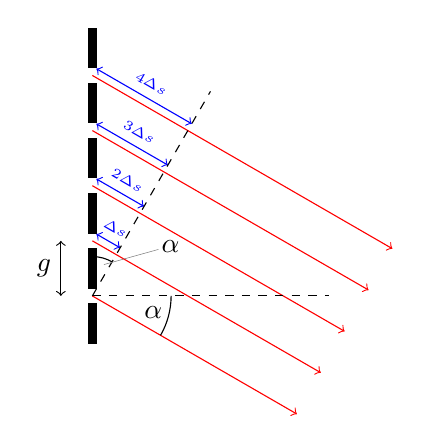
\begin{tikzpicture}
  \pgfmathsetmacro{\gratinglength}{0.7};
  \pgfmathsetmacro{\gratingwidth}{0.1};
  \pgfmathsetmacro{\gratingdistance}{0.2};
  \pgfmathsetmacro{\angle}{-30};
  % grating
  \foreach \Y in {0,\gratinglength,...,4.0} {%
    \draw[fill] ({-\gratingwidth/2},\Y) rectangle ({\gratingwidth/2},\Y+0.5);
  }
  % rays
  \foreach \m in {0,...,4} {%
    \draw[red,->] (0,{\m*\gratinglength + (\gratinglength - \gratingdistance/2)}) -- ++ ({\angle}:{3+\m*\gratinglength*sin(30)});
  }
  % distances
  \begin{scope}[shift={(0,{\gratinglength - \gratingdistance/2})},rotate={\angle}]
    \draw[<->,blue] (0,{\gratinglength*cos(\angle)+0.1}) -- ++ ({\gratinglength*sin(\angle)},0) node[midway,above,rotate={\angle}] {\tiny $\Delta s$};
    \foreach \m in {2,...,4} {%
      \draw[<->,blue] (0,{\m*\gratinglength*cos(\angle)+0.1}) -- ++ ({\m*\gratinglength*sin(\angle)},0) node[midway,above,rotate={\angle}] {\tiny $\m\Delta s$};
    }
  \end{scope}
  % angle 1
  \coordinate (O) at (0,{\gratinglength - \gratingdistance/2});
  \coordinate (R) at ($(O)+({\angle}:{3+\gratinglength*sin(30)})$);
  \draw[dashed] (O) -- ++ (3,0) coordinate (A1);
  \pic[draw,pic text={$\alpha$},angle radius=1cm,angle eccentricity=0.8] {angle = R--O--A1};
  % angle 2
  \coordinate (G) at (0,1);
  \draw[dashed] (0,0.6) -- ++ (60:3) coordinate (A2);
  \pic[draw,pic text={},pic text options={pin={[pin distance=2em]10:{$\alpha$}}},inner sep=1pt,angle radius=0.5cm,angle eccentricity=0.8] {angle = A2--O--G};
  %
  \draw[<->] (-0.4,{\gratinglength - \gratingdistance/2}) -- node[left] {$g$} ++ (0,{\gratinglength});
\end{tikzpicture}
\end{document}
